\documentclass[a4paper,11pt,twocolumn]{article}
\pagestyle{myheadings}
\usepackage[utf8]{inputenc}
\usepackage[letterpaper,margin=0.5in]{geometry}
\usepackage[T1]{fontenc}
\usepackage{tgbonum}
\usepackage{csquotes}
\usepackage{enumitem}
\usepackage{parskip}
\usepackage{titlesec}
\usepackage{hyphenat}
\usepackage{fancyhdr}
\usepackage{tabularx}
\usepackage{multirow}
\usepackage{authblk}
\usepackage{xcolor,colortbl}
\usepackage{graphicx}
\usepackage{tocloft}

\graphicspath{
  {./Images/Counters/},
  {./Images/Misc}
}

\title{%
    Hastings: 1066 \\
    \vspace{0.5em}
    \large Strategy \& Tactics Magazine, Nr. 110, 1986}
\author{Designed by: Richard Berg}
\affil{This document created by: Daniel Berger}

\setlength{\columnsep}{2em}
\setcounter{secnumdepth}{4}

\pagestyle{fancy}
\fancyhead{}
\fancyfoot{}
\fancyfoot[R]{Page \thepage}

\titlespacing{\paragraph}{0pt}{1em}{\medskipamount}

\titleformat
  {\section}
  [runin]
  {\LARGE}
  {[\thesection.0]}
  {0.5em}
  {}

\titleformat
  {\subsection}
  [hang]
  {\bfseries}
  {[\thesubsection]}
  {1em}
  {}

\titleformat
  {\subsubsection}
  [runin]
  {\bfseries}
  {[\thesubsubsection]}
  {1em}
  {}

\newenvironment{hangsubsubsection}
{
  \titleformat
  {\subsubsection}
  [hang]
  {\bfseries}
  {[\thesubsubsection]}
  {1em}
  {}
}
{
  \titleformat
  {\subsubsection}
  [runin]
  {\bfseries}
  {[\thesubsubsection]}
  {1em}
  {}
}

\newenvironment{noverticalspace}
{%
  \par % ensure we're in vertical mode
  \offinterlineskip % don't do the baselineskip calculations
}
{\par}% be sure to finish up

\definecolor{BabyBlue}{rgb}{0.54, 0.81, 0.94}

\renewcommand{\contentsname}{Hastings 1066 - Table of Contents}
\setcounter{tocdepth}{2}
\setlength{\cftsecindent}{0em}

\begin{document}
\maketitle
\section{INTRODUCTION}
\hfill

The \textit{Hastings: 1066} game is a tactical simulation of the confrontation between William the Bastard, Duke of Normandy, and King Harold Godwineson of Wessex, a battle that forever changed the face of the world. William and his combined force of Normans, Bretons, French and Flemings, is moving on London. His way is blocked by the hastily assembled Saxon army of Harold, fresh from victory over the Danes at Stamford Bridge. The victor will be king of England.

In this game, the armies are divided into \textit{nationalities} (Normans) or \textit{wings} (Saxons). The ability of each nationality or wing to move and attack is restricted by the formation or \textit{order} it adopts. These are influenced by the \textit{strategy} each player selects at the start of each game turn. Over the course of the battle, the choice of strategy will cummulatively affect the fatigue level and morale of the troops. The details of this process are given in Section 4.0 of these rules.
\section{GAME PARTS}

\subsection{The Game Map}

The 17" by 22" mapsheet represents the battlefield at Hastings (actually Senlac Hill; Hastings is some miles to the south). The map is covered by a hexagonal grid to regulate movement and combat. The types of terrain and their effects are listed on the Terrain Effects Charts and in Section 5.3.

\subsection{The Playing Pieces}

The playing pieces, or counters, represent the forces (units) and commanders (leaders) involved in the battle. Certain other pieces (markers) are used to record unit status, time, and other game functions.

Historically, Williams's army included not only Normans, but Breton and Franco-Flemish contingents as well. Unless specifically stated otherwise, the term "Norman" refers to William's entire army.

\textcolor{teal}{Note: The unit images displayed here are of my own creation. While they are very similar to the units that are included in the physical game, there are some minor differences and additions, such as the inclusion of a facing arrow and the MP rating on the back of a flipped leader.}

\begin{center}
\textbf{LEADER UNIT}
\break
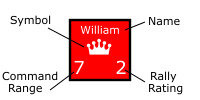
\includegraphics{Markers/Leader_Description.jpg}
\break
\break
\textbf{COMBAT UNITS}
\break
\break
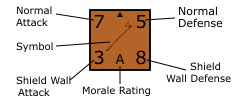
\includegraphics{Markers/Foot_Unit_Description.jpg}
\par
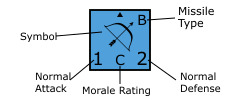
\includegraphics{Markers/Missile_Unit_Description.jpg}
\end{center}
\break

\renewcommand\tabularxcolumn[1]{m{#1}}

\par
\begin{center}
  \textbf{SUMMARY OF LEADER UNIT TYPES}
  \break
\end{center}

\begin{tabularx}{0.5\textwidth}{
    >{\raggedright\arraybackslash}X
    >{\centering\arraybackslash}X
    >{\raggedleft\arraybackslash}X}
    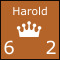
\includegraphics{Saxons/Harold.jpg} &
    \textbf{Kings} &
    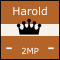
\includegraphics{Saxons/Harold_Ineffective.jpg} \\ \\
    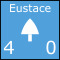
\includegraphics{Normans/Eustace.jpg} &
    \textbf{Leaders} &
    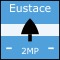
\includegraphics{Normans/Eustace_Ineffective.jpg}
\end{tabularx}

\par
\begin{center}
  \textbf{SUMMARY OF COMBAT UNIT TYPES}
  \break
\end{center}

\begin{tabularx}{0.5\textwidth}{
    >{\raggedright\arraybackslash}X
    >{\centering\arraybackslash}X
    >{\raggedleft\arraybackslash}X}

  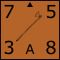
\includegraphics{Saxons/Housecarle.jpg} & \textbf{HouseCarles} & 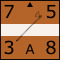
\includegraphics{Saxons/Housecarle_Ineffective.jpg} \\ \\
  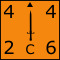
\includegraphics{Saxons/Thegn.jpg} & \textbf{Thegns} & 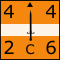
\includegraphics{Saxons/Thegn_Ineffective.jpg} \\ \\
  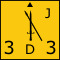
\includegraphics{Saxons/Great_Fyrd_1.jpg} & \textbf{Great Fyrd} & 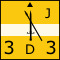
\includegraphics{Saxons/Great_Fyrd_1_Ineffective.jpg} \\ \\
  
\includegraphics{Saxons/Great_Fyrd_2.jpg} & \textbf{Great Fyrd} & 
\includegraphics{Saxons/Great_Fyrd_2_Ineffective.jpg} \\ \\
  
\includegraphics{Saxons/Slingers.jpg} & \textbf{Slingers} & 
\includegraphics{Saxons/Slingers_Ineffective.jpg} \\ \\
  
\includegraphics{Normans/Norman_Cavalry.jpg} & \textbf{Norman Knight} & 
\includegraphics{Normans/Norman_Cavalry_Ineffective.jpg} \\ \\
  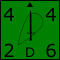
\includegraphics{Normans/Breton_Infantry.jpg} & \textbf{Breton Foot} & 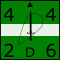
\includegraphics{Normans/Breton_Infantry_Ineffective.jpg} \\ \\
  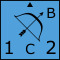
\includegraphics{Normans/Franco-Flemish_Bowmen.jpg} & \textbf{Fr-Flemish Bowmen} & 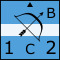
\includegraphics{Normans/Franco-Flemish_Bowmen_Ineffective.jpg}
\end{tabularx}

\break

\par
\begin{center}
  \textbf{SUMMARY OF MARKER TYPES}
  \break
  \par
  \textbf{Strategy Markers}
\end{center}

\begin{tabularx}{0.5\textwidth}{
    >{\raggedright\arraybackslash}X
    >{\centering\arraybackslash}X
    >{\raggedleft\arraybackslash}X}
  
\includegraphics{Markers/Norman/Aggressive_Strategy_Norman.jpg} &
  \textbf{Strategy Marker} &
  
\includegraphics{Markers/Norman/Cautious_Strategy_Norman.jpg} \\ \\
  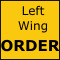
\includegraphics{Markers/Saxon/Saxon_Left_Wing_Order.jpg} &
  \textbf{Order Marker} &
  
\includegraphics{Markers/Saxon/Saxon_Right_Wing_Order.jpg} \\ \\
  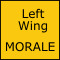
\includegraphics{Markers/Saxon/Morale_Left_Wing_Saxon.jpg} &
  \textbf{Morale Marker} &
  
\includegraphics{Markers/Saxon/Morale_Right_Wing_Saxon.jpg} \\ \\
  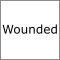
\includegraphics{Markers/Wounded.jpg} &
  \textbf{Wounded/Shaken Marker} &
  
\includegraphics{Markers/Shaken.jpg} \\ \\
  
\includegraphics{Markers/Disrupted.jpg} &
  \textbf{Disrupted/Routed Marker} &
  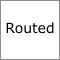
\includegraphics{Markers/Routed.jpg}
\end{tabularx}


\subsection{Game Charts and Tables}


The charts and tables simplify and illustrate certain game mechanics. These are the Norman and Saxon Order Tables, the Terrain Effects Chart, the Missile Fire Matrix, the Missile Fire Results Table, the Melee Results Table, the Morale Table, the Rally Table and the Leader Casualty Table. The locations and use of these charts and tables are noted in the appropriate rule sections.

\subsection{Game Tracks and Displays}

The tracks and displays used in the game are used to record unit status and the progress of the game. They include the Norman and Saxon Strategy Displays, the Norman and Saxon Order Displays, the Assault Period Display, the Battle Turn Record Track, and the Norman and Saxon Strategy Effect Tracks. These are located on the game map.

\subsection{Game Scale and Playing Time}

Each hex on the game map covers approximately 45 yards. Each housecarl or bowman unit represents about 100 men; all other units represent about 125-150 men. Each Assault Period should take from three to four hours to complete and covers several hours of real time. (Historians should note that the four separate phases of the actual battle have been reduced to two Assault Periods for play purposes.)

\subsection{Inventory of Game Parts}

A complete game includes:

\begin{enumerate}[label=*]
    \item One 17" x 22" game map
    \item One rule booklet
    \item 200 die-cut counters
\end{enumerate}

In addition, two six-sided dice must be provided by the players.
\section{SEQUENCE OF PLAY}
\hfill

Each game consists of two Assault Periods, each consisting of eight Battle Turns. At the beginning of every turn, each player chooses a strategy that will affect the battle order adopted by various parts of his army for that turn.

\subsection{The Assault Period}

Each Assault Period consists of eight Battle Turns. At the end of the First Assault Period, the players check to see if the Assault Period is extended (3.3). If not, the armies are reorganized (11.5) and the Second Assault Period begins. The game ends at the conclusion of the Second Assault Period unless one player has previously achieved his victory conditions (12.0).

\subsection{The Battle Turn}

Each Battle Turn consists of an Order Phase, a Norman Player Phase, a Saxon Player Phase and a Turn Record Phase. The player who is active in the phase is called the \textit{phasing player}; the inactive player is called the \textit{non-phasing player}.

ORDER PHASE

At the beginning of every Battle Turn, each player selects a strategy for that turn (4.2). He then consults his Order Table and rolls two dice for each wing or nationality of his army to determine which battle order it will adopt for that turn. Both players can perform this phase simultaneously.

NORMAN PLAYER PHASE

\begin{enumerate}
    \item \textbf{Rally Segment:} The Norman player attampts to rally his disrupted/routed units. Any routed units that fail to rally must immediately move two hexes to the rear.
    \item \textbf{Norman Missile Segment:} Norman missile units can fire at any enemy units within range. Casualties are taken as they occur.
    \item \textbf{Norman Movement Segment:} All unrouted and undisrupted Norman units can move if their order allows.
    \item \textbf{Saxon Reaction Segment:} Non-phasing Saxon units in proper order can move according to the rules governing reaction (5.4).
    \item \textbf{Saxon Missile Segment:} Non-phasing Saxon missile units can fire at any enemy units within range. Only bowman units can fire after taking a reaction move.
    \item \textbf{Melee Segment:} The Norman player melees all Saxon units exerting \textit{zones of control} (5.7) on his units. Casualties are taken immediately, then any units that must retreat must do so.
\end{enumerate}

THE SAXON PLAYER PHASE

The Saxon player repeats 1-6 above, with the Saxon and Norman player reversing roles.

TURN RECORD PHASE

At the end of the Saxon Player Turn, the players advance the Battle Turn Marker on the Turn Record Track. At the end of the First Assault Period, if no decision has been reached, the players reform their armies (see 11.5) and advance the Assault Period Marker on the Assault Period Display, returning the Battle Turn Marker to the beginning of the Turn Record Track. At the end of the second period, the game is over.

\subsection{The Extended Assault Period}

\subsubsection{} The standard Assault Period lasts eight Battle Turns. However, under the following circumstances the Assault Period can be extended:

\begin{enumerate}[label=*]
    \item If more than 50\% of the Norman combat units are on Senlac Hill at the end of the eighth Battle Turn, the period is extended \textit{two} more turns.
    \item If more than 75\% of the Norman combat units are on Senlac Hill at the end of the eighth Battle Turn, the period is extended \textit{three} more turns.
    \item If \textit{all} undisrupted, unrouted Saxons are entirely surrounded by Norman units, Norman zones of control, or the map edge, the period is extended until the Normans win or the encirclement is broken.
\end{enumerate}

Only one of these conditions can be applied at any time; they are mutually exclusive. If there is any question, the Norman player chooses. The Assault Period Marker can be placed on the Turn Record Track to mark the end of the extended period.

\subsubsection{} In an extended period, the following special conditions apply:

\begin{enumerate}[label=*]
    \item The Norman player can reroll any Shield Wall and Hold order he rolls if desired (in this case the Norman player can roll separately for the foot or knight section of a ntionality); and
    \item The Saxon player can reroll any Attack \& Pursue order he rolls if desired.
\end{enumerate}

\subsection{Assault Period Display}

\begin{center}
  
\includegraphics[scale=0.35]{Assault_Period.png}
\end{center}

\subsection{Battle Turn Record Track}

\begin{center}
    
\includegraphics[scale=0.3]{Battle_Turn_Record_Track.png}
\end{center}
\section{STRATEGY AND BATTLE ORDER}
\hfill

GENERAL RULE:

In the Order Phase of every Battle Turn, each player selects a basic strategy for each wing or nationality in his army for the ensuing Battle Turn. The Order Tables simulate the general inefficiency and lack of control that plagued medieval commanders.

\subsection{Wings and Nationalities}

Each player's army is divided into \textit{wings} (Saxons) or \textit{nationalities} (Normans) for determining battle order. Norman nationalities are further divided into \textit{sections} of foot and knights.

\subsubsection[Saxon Wings]{}

The Saxon Army initially consists of three wings - right, center and left - each commanded by a leader. The leader's command radius usually determines which units make up his wing.

\subsubsection[Defining Saxon Wings]{}

Wings are defined at the beginning of each individual Battle Turn. No Saxon leader can control less than 20\% (1/5) of the Saxon units available. A given leader can control any number of units within his command radius as long as no Saxon leader controls less than 20\% of the Saxon units.

\subsubsection[Saxon Leader Loss and Wings]{}

If the Saxons are reduced to less than three leaders, no leader can control less than 33\% (1/3) of the Saxon units. If a Saxon leader dies during a Battle Turn, his wing is what it originally was until its units come under the control of the remaining Saxon leaders. If the Saxons have no leaders, they are assumed to have only one wing.

\subsubsection[Norman Sections]{}

The Norman army has six sections: Norman Foot/Bowmen, Norman Knights, Breton Foot/Bowmen, Breton Knights, Franco-Flemish Foot/Bowmen, and Franco-Flemish Knights. William's personal guard is \textit{not} part of any section (see 4.38). Norman leaders do not define Norman sections.

\subsubsection[Leaders and Unit Orders]{}

Leaders never affect the order of their units. An army can operate without leaders, albeit with reduced efficiency.

\subsubsection[Define Wings and Sections]{}

Players must always clearly define their wings and sections. Certain situations can make this difficult. Try to establish what is what before you proceed, and treat this rules section liberally in that respect.

\subsection{Strategy}

Specific strategies are chosen for each wing or nationality for each Battle Turn. These will influence, but not control, the order adopted by the units of the wing or sections of the nationality for the turn (medieval troops were notoriously difficult to control). The strategy used will have a long-term effect on friendly morale and endurance.

\subsubsection[Strategies]{}

There are four strategies available: Defensive, Cautious, Moderate, and Aggressive. The player can choose a different (or the same) strategy for each of his wings or nationalities. Each player has a number of Strategy markers corresponding to the available strategies.

\subsubsection[Strategy Display]{}

Each player has a Strategy Display on the game map. In the Order Phase of each Battle Turn, the player places face-down in each box a Strategy marker corresponding to his selected strategy for that wing or nationality. The strategies are not revealed until the players are ready to determine their battle order.

\subsubsection[Order Tables]{}

After a strategy has been chosen for each wing/nationality, the players consult the Order Tables printed on the map. Each player rolls two dice for each wing/nationality and compares the roll to the strategy selected for that wing/nationality to find out what order it will adopt during the ensuing Battle Turn. The order rolled is applied to all units in that wing or section (see 4.24). An Order Marker is placed in the appropriate box on the player's Order Display (printed on the map), indicating the order in effect for the turn. The Morale marker for that wing or section is adjusted on the Strategy Effects Table.

\textcolor{blue}{When determining the Norman Strategy Effect from the Battle Order Determination Table (4.46) the separate effects of the Knights and the Foot are combined (i.e. they are cumulative) for a given nationality. Thus a -2 and a +1 would produce an effect for that turn of -1.}

\subsubsection[Orders]{}

The Saxon player rolls for each existing wing. The Norman player rolls for each \textit{nationality} (Norman, Breton, and Franco-Flemish). \textbf{Important:} This roll is read separately for both the knight and foot units of their nationality.

\subsubsection[Leaders and Orders]{}

Leaders never adopt an order; they are not affected by these rules.

\subsubsection[Order Length]{}

Some orders last for two turns. Wings/sections in those orders ignore theorder dice roll. Instead, their marker is moved from the "2" turn box to the "1" turn box on the player's Order Display.

\subsubsection[Optional Order]{}

A result of \textbf{Optional} means that the player chooses the order desired for that wing/section for the phase.

\subsection{Battle Order}

\textit{The following battle order descriptions (4.31 through 4.34) are adopted only by foot units.}

\subsubsection{Shield Wall:} Non-bow foot units in this order use their \textit{Shield Wall} combat strengths. They are not required to attack (an exception to 8.12). Their movement allowance is "0"; however, units using thsi order can move one hex towards the rear (9.23) as long as they do not enter an enemy zone of control. Units in Shield Wall order cannot "react" as per 5.4.

Bowmen never adopt a Shield Wall order; if this order is in effect, bowmen (only) adopt Melee/Fire in Place instead.

\subsubsection{Melee/Fire in Place:} Units use their normal combat strengths and can fire and melee normally. Units in this order have a movement allowance of "0", but may either advance or retreat one hex as long as they do not enter an enemy zone of control.

\subsubsection{Advance to Combat:} All combat strengths and movement allowances are normal and unrestricted. Movement is voluntary for each unit Units need not move toward the enemy.

\subsubsection{Attack \& Pursue \textit{(Saxon foot only)}:} Any unit in this order must, where possible, move toward the nearest enemy unit. Units in this order not adjacent to the enemy must move as close to such units as possible; those in an enemy zone of control can move, so long as they end their movement adjacent to an enemy unit. In addition:

\begin{itemize}
  \item Units in this order cannot move in the friendly reaction segment.
  \item During melee, normal combat strengths are used. \textbf{D} combat results inflicted by units in this order become \textbf{R} results. Units in this order routing an enemy unit \textit{must} pursue, as detailed in Case 9.4.
  \item The Attack \& Pursue order remains in effect for the number of Battle Turns given on the Order Table.
\end{itemize}

\textit{The following orders are adopted only by Norman knights of any nationality:}

\subsubsection{Hold:} This is the same as the Shield Wall order, except that the knights use their normal combat strength.

\subsubsection{Advance:} This is the same as 4.33.

\subsubsection{Charge:} This is a voluntary order that allows knight units to increase their combat strengths under certain conditions. If the conditions cannot be met, or if the Norman player does not wish to charge, the individual knight unit will be in the Advance to Combat order. Charge conditions are:

\begin{itemize}
  \item The charge must end in contact with an enemy unit.
  \item The charge cannot cross a ridge or stream hexside, or enter a marsh or woods hex.
  \item The last two hexes of the charge cannot be uphill (see 5.33).
\end{itemize}

When charging, knights have a movement allowance of \textit{six} and all knight units in the section (whether actually charging or not) must move toward the enemy, as described in 4.34. In addition:

\begin{itemize}
  \item Units in this order cannot move in a friendly reaction segment.
  \item In melee, a successfully charging knight unit adds \textit{one} to its combat strength; \textit{two} if charging downhill.
  \item All \textbf{D} results inflicted by charging knights are treated as \textbf{R} results (see 9.1). After a successful charge (and subsequent melee) the knight unit must undergo a morale check (see 9.62) regardless of any other combat result. Routed enemy units must be pursued by undisrupted knights as per 9.4.
  \item A Charge order remains in effect for the number of turns given on the Order Table.
\end{itemize}

\textcolor{blue}{If a Knight unit receives a Charge order, but does not meet the conditions for Charging (the three conditions listed at the beginning of the section), it may still increase its movement rate (to 6 MPs); however, if it attacks, it uses its printed attack strength (it does not receive the +1/+2 Charge bonus). All other effects apply, however, as if the Charge were allowed.}

\subsubsection[Exceptions to Order Rules]{} The following situations are exceptions to the order rule:

\begin{enumerate}
  \item \textbf{William's Guard:} This knight unit (distinguished by its "A" morale) is free to move as desired by the Norman player - as long as William is alive. It is not affected by the order rules and may charge at any time, as long as it meets the charge requirements. If William is dead, the unit becomes part of the Norman knight section.
  \item \textbf{Saxon Reinforcements:} When entering the game as per 12.3, these units are in Advance to Combat order until they come within the command radius of a leader \textit{or} move adjacent to an enemy unit. At this point they are arbitrarily assigned to the nearest wing.
  \item \textbf{Harold's Housecarls (optional rule):} Historically the Saxon housecarls were less impetuous than the fyrd, who tended to charge recklessly into combat. Thus, the housecarls treat an Attack \& Pursue order as an Optional order. The Saxon player, however, must make this decision prior to his order dice roll and cannot change his mind after the roll is made. \textit{(This rule greatly favors the Saxons and can be used as a balancing element)}
\end{enumerate}

\subsection{Displays and Tables} \textit{(see map)}

\subsubsection{Saxon Strategy Display}

\subsubsection{Saxon Battle Order Determination Table}

\subsubsection{Saxon Battle Order Display}

\subsubsection{Saxon Strategy Effects Track}

\subsubsection{Norman Strategy Display}

\subsubsection{Norman Battle Order Determination Table}

\subsubsection{Norman Battle Order Display}

\subsubsection{Norman Strategy Effects Track}
\hfill

\textcolor{blue}{At the beginning of the game, all ratings on the Strategy Effects Track start at "0". Additionally, at the start of the second Assault Period, return all ratings back to "0".}

\section{Movement}

GENERAL RULE:

During the movement segment of a Battle Turn, the phasing player can move as many or as few of his units as he wishes, in any direction or combination of directions. Each unit has a \textit{movement allowance} (5.12) that can be restricted by its Battle Order. Normally, however, each unit can spend as many of its movement points (MPs) as desired within the limits of its movement allowance.

\pagebreak
PROCEDURE:

Units are moved one at a time, tracing a path of contiguous hexes through the hex grid. As a unit enters a hex or crosses a hexside, it must pay part of its movement allowance. These costs are listed on the Terrain Effects Chart on the map.

\subsection{How to Move}

\subsubsection[Movement Calculation]{} Movement is calculated in terms of hexes. Basically, each unit spends one movement point for each hex that it enters. Some hexes and hexsides cost additional movement points to enter or cross, as listed on the Terrain Effects Chart.

\subsubsection[Movement Costs]{} The movement costs for all units are as follows:

\begin{tabular}{ |l|l| }
  \hline \\ [-2.0ex]
  & \textbf{Movement} \\
  \textbf{Unit} & \textbf{Allowance} \\
  \hline \\ [-2.0ex]
  Knights (Cavalry) & 4 MP (normal) \\
  & 6 MP (charging) \\
  Leader & 6 MP \\
  All Others (Foot, Bowmen, etc) & 3 MP \\
  \hline
\end{tabular}

These are the \textit{maximum} number of movement points the unit can use within a given movement segment. \textit{See 4.3 for battle order restrictions on movement allowances.}

\subsubsection[Movement Limits]{} Units can be moved only once in a movement segment. However, certain movement (such as rout, pursuit and reaction) is not considered movement under this section. Rout (9.23) and pursuit (9.4) do not use movement points, nor are they restricted by battle order. Reaction does not use movement points, but \textit{is} restricted by battle order.

\subsubsection[Movement Point Use]{} No unit is required to use all (or any) of its allotted movement points. However, unused movement points cannot be transferred from unit to unit, nor can they be saved for the next movement segment.

\subsubsection[Movement and Facing]{} Units can move into any hex for which they have the movement points available (5.21). The \textit{facing} of a unit (6.0) does not affect its movement (however, see 6.11). Leaders have no effect on movement.

\subsection{Restrictions on Movement}

\subsubsection[Moving Through Units]{} All units can always move through other friendly units. Combat units cannot end their movement in the same hex as another combat unit. Leaders can end their movement in the same hex with other friendly units. Friendly units cannot enter an enemy-occupied hex.

\subsubsection[Movement and Combat]{} There is no combat during movement, and enemy units cannot move in a friendly movement segment.

\subsubsection[No Skipping]{} Movement from hex to hex must be consecutive; units cannot "skip" hexes.

\subsubsection[Movement During Fire and Melee]{} There is usually no movement during the fire or melee segments. However, certain combat results call for a rout or pursuit, in which case the affected units are moved according to rules 9.23 and 9.4.

\subsubsection[Battle Order Limits]{} Certain battle orders limit the movement allowances of units that adopt them (see 4.3).

\subsection{The Effects of Terrain on Movement}

\subsubsection[Hex Costs]{} Each hex - and certain types of hexsides - have a specific movement point cost to enter or cross (see the Terrain Effects Chart).

\subsubsection[Terrain Color]{} The color of a hex on the game map represents its approximate elevation; the darker hued the hex, the higher the elevation. Terrain features are represented by symbols in the hex or along the hexside. For example, the slopes hexsides that separate certain elevations represent relatively sharp increases in height. A given hex is always the height of the highest elevation in that hex.

\subsubsection[Uphill]{} The term "uphill" means any movement that either goes from a lower elevation to a higher elevation \textit{or} any movement that takes a unit within \textit{two} hexes of a higher elevation moving in the direction of the higher elevation. There are two exceptions:

\begin{itemize}
  \item Movement within two hexes of the hill in hex 1419 or the "top" of Senlac Hill (275 foot elevation) does not count as uphill. Units must actually move \textit{into} these hexes or the upslope hexes of the hill to be moving uphill; and
  \item Units moving laterally to or away from a higher elevation are not moving uphill, regardless of the hex they are in. Thus, a unit moving from 0918 to 0919 or 0920 is not moving uphill.
\end{itemize}

\subsubsection[Downhill]{} "Downhill" is the reverse of uphill; using the precepts of 5.33, but with the direction reversed.

\subsubsection[Norman Knights]{} Each time a Norman knight unit tries to cross a ridge while moving in \textit{any} direction, the knight unit undergoes an immediate morale check in the hex preceding the ridge, treating all routs as disruptions. If the knight unit does not become disrupted, its movement ends. It remains in the hex until rallied or moved in a later segment. If undisrupted, it continues its move normally.

\subsubsection[Knights and Marsh]{} Each time a knight unit enters a marsh hex it must undergo an immediate morale check as detailed in 5.35. Again, all routs are treated as disruptions.

\subsubsection[The Road]{} The road has no effect on movement or combat.

\subsection{Reaction}

\subsubsection[Reaction Defined]{} Reaction is a form of movement used only by the non-phasing player. Reaction movement occurs only in the reaction segment of the other player's phase.

\subsubsection[How Reaction Works]{} Units capable of reaction (see 5.44) can, if desired, move \textit{one} hex away from an enemy combat unit during a friendly reaction segment. Such movement does not use or cost movement points; moreover, terrain has no effect on such movement.

\subsubsection[Reaction and ZOCs]{} Units using reaction cannot move into enemy zones of control (ZOC).

\subsubsection[Eligible Units]{} Only eligible units can use reaction. All units are eligible except the following:

\begin{enumerate}
  \item Saxon foot units in the ZOC of an enemy (mounted) Knight.
  \item Any unit in the following order: Shield Wall, Attack \& Pursue, or Charge.
  \item Any unit not in the command range of a friendly leader.
\end{enumerate}

\subsubsection[Morale Check]{} Any unit that uses reaction undergoes a morale check upon completing the movement.

\subsubsection[Missile Fire]{} A unit using reaction cannot use missile fire in the following defensive missile fire segment, unless the moving unit is a bowman unit. Bowman units can both react and fire.

\subsection{Terrain Effects Chart}

\resizebox{\columnwidth}{!}{
\begin{tabular}{ |ccl| }
  \multicolumn{3}{c}{\textbf{Terrain Effects Chart}} \\
  \hline & &\\[-2.0ex]
  \textbf{Terrain Type} & \textbf{Movement Cost} & \textbf{Effect on Combat} \\
  \hline & & \\[-2.0ex]
  Clear & 1 MP & None \\
  \rowcolor{BabyBlue}
  & & Foot: -1 Melee\\
  \rowcolor{BabyBlue}
  \multirow{-2}{*}{Ridge, Uphill} & \multirow{-2}{*}{None*} & Knight: -2 Melee \\
  & & Foot: +1 Melee \\
  \multirow{-2}{*}{Ridge, Downhill} & \multirow{-2}{*}{None*} & Knight: None \\
  \rowcolor{BabyBlue}
  & & Foot: None \\
  \rowcolor{BabyBlue}
  \multirow{-2}{*}{Movement Downhill} & \multirow{-2}{*}{None*} & Knight: +1/+2 Melee \\
  \multirow{2}{*}{Marsh} & Foot: 2 MP & \multirow{2}{*}{-1 Def} \\
  & Knight*: 3 MP & \\
  \rowcolor{BabyBlue}
  Stream & +1 MP & None \\
  \multirow{2}{*}{Woods} & Foot: 2MP & +2 in Melee/+1 vs Bow \\
  & Knight: 3 MP & (for units in woods)\\
  \rowcolor{BabyBlue}
  Road & 1 MP & None \\
  \hline
\end{tabular}
}

* Knights: Morale Check. Treat rout as disrupt.

\subsection{Stacking}

\subsubsection[Limits]{} Only one combat unit can end a movement, fire or melee segment in any one hex. Leaders can always stack with friendly units. Informational markers can also be placed in hexes with other counters.

\subsubsection[Moving Through Units]{} Friendly units of all types can freely pass through each other during movement, reaction, rout, pursuit, etc.

\subsubsection[Knights and Stacking]{} A knight unit cannot be moved into an occupied hex if such movement would cause a morale check (see 5.35 and 5.36). This is an exception to 5.62.

\subsection{Zones of Control}

All combat units that are not disrupted or routed exert a zone of control (ZOC) through their frontal hexsides into adjacent hexes. Such hexes are \textit{controlled} by the units exerting the ZOC. Leaders and routed units do not exert ZOC's. ZOC's are not affected by terrain. ZOC's themselves affect movement and combat.

\subsubsection[Stopping Movement]{} A unit must stop whenever it enters an enemy-controlled hex. It can move no further in that movement segment. A combat unit cannot enter an enemy ZOC that is occupied by another friendly combat unit.

\subsubsection[Leaving a ZOC]{} Friendly units beginning a movement segment in an enemy ZOC can leave the ZOC as long as they do not move directly into another enemy-controlled hex. Such units may eventually enter an enemy-controlled hex in the same segment as long as the movement is not directly from one enemy ZOC to another.

\subsubsection[Bowmen and ZOCs]{} Bowmen untis can never voluntarily enter an enemy ZOC. Such units in an enemy ZOC at the start of a friendly movement segment must move out of the ZOC if they can. There is no penalty if they are unable to do so.

\subsubsection[MP and ZOCs]{} There is no additional movement point cost to enter or leave enemy ZOC.

\subsubsection[Competing ZOCs]{} If both friendly and enemy units exert a ZOC into the same hex, both units control the hex. There is no additional effect for having more than one unit control a hex.

\subsubsection[Friendly ZOCs]{} Friendly ZOC's never affect friendly units.

\subsubsection[ZOCs and Combat]{} The effects of ZOC's on combat are given in 6.24 and 8.11.

\section{FACING}
\hfill

GENERAL RULE:

After finishing all movement, all combat units must be \textit{faced} (oriented) in a specific direction. The facing of a unit affects its ability to attack and defend. Facing affects movement or reaction only when the unit is routed. Leader units are not subject to the facing rules.

\subsection{How Units Are Faced}

\subsubsection[Facing Direction]{} All combat units must be faced in a specific direction after they finish movement and maintain that facing until they move again. Facing does not use movement points. A unit that is eligible to move and does not can still change its facing.

\subsubsection[Combat Units]{} Combat units are faced so the top of the unit points to a vertex of its hex. Each unit has two \textit{frontal}, two \textit{flank} and two {rear} hexsides.

\subsubsection[Battle Order]{} Battle order never affects facing.

\subsection{Effects of Facing on Combat}

\subsubsection[Missile Armed Troops]{} Missile-armed units can fire only through their frontal hexsides,

\subsubsection[Melee]{} Units can melee only those enemy units that are in their frontal (controlled) hexsides. A unit must attack all enemy units in its ZOC, unless the enemy unit is being meleed by another friendly unit.

\subsubsection[Flank or Rear]{} Friendly units attacking the flank or rear hexsides of an enemy unit receive a bonus to their combat rating (either fire or melee), as given.

\begin{tabular}{ lcc }
  & \textbf{Flank} & \textbf{Rear} \\
  \hline
  Fire & +1 & +1 \\
  Melee & +1 & +2 \\
\end{tabular}

Thus, a Breton foot unit in Advance to Combat order meleeing a Saxon fyrd unit through the fyrd's rear hexside would have a melee rating of “6” rather than its printed rating of “4".

\subsubsection[Defensive Ratings]{} Defensive ratings do not change if the unit is attacked through its flank or rear. Thus, a housecarle unit in Shield Wall order meleed from the rear would defend with its Shield Wall strength of “8.”
\section{MISSILE FIRE COMBAT}
\hfill

GENERAL RULE:

Any unit with missile capability (see Sample Units, 2.2) can fire in a friendly fire segment. Such units can fire at any enemy units within the range allowed on the Missile Fire Matrix. Bowmen units (only) can use \textit{high trajectory fire} to shoot over friendly units or enemy units. There are restrictions on the ability to fire, as well as the number of times a missile unit can fire.

PROCEDURE:

During a friendly missile fire segment, the firing player determines which of his eligible missile units will fire at which enemy units. Using the Missile Fire Matrix, he cross references the unit type (bowman, javelin or sling) with the range in hexes from the enemy target. The resultant number is the \textit{fire strength} of the firing unit for that attack.

The player totals the fire strengths of all units firing at a given enemy unit and compares the total to the enemy unit's \textit{defensive strength} (which depends on the battle order in effect). Adjustments for terrain and high trajectory are taken, and the comparison is stated as a simple \textit{odds ratio} of attacker to defender. All odds are rounded off in favor of the defender; thus 10 to 3 is reduced to 3-1.

The firing player rolls one die and cross-references the die roll with the odds ratio on the Missile Fire Combat Results Table. Any result is applied immediately.

\subsection{How to Engage in Missile Combat}

\subsubsection[Missile Capability]{} Only units with a \textit{missile capability letter} can attack with missiles (see sample units, 2.2).

\subsubsection[Missile Strength]{} To find a unit's fire strength, the player counts the number of hexes to the target unit, excluding the firing unit's hex but including the target unit's hex. He then cross-references this range with the type of unit firing (on the Missile Fire Matrix, see map) to get that unit's fire strength. Note that the maximum ranges for each type of missile unit are limited.

\subsubsection[Combined Fire]{} Missile units can combine their strengths when firing at a given target, the strength contributed by each depending on range. An individual unit cannot split its fire strength between two or more hexes.

\subsubsection[Missile Procedure]{} After determining the total fire strength, missile fire proceeds as stated in the Procedure, above.

\subsubsection[Melee and Missile]{} Units can engage in missile fire the same turn in which they melee.

\subsubsection[Missile Fire Results]{} The Missile Combat Results Table (see map) has three results:

\begin{itemize}
  \item \textbf{M = Morale Check}. The affected unit undergoes an immediate \textit{morale check} (see 9.6).
  \item \textbf{D = Disrupted}. Place a Disrupted Marker on the unit to indicate its disrupted status (see 9.22).
  \item \textbf{1 = Reduced}. The affected unit is flipped over to indicate its reduced status. If already reduced, it is eliminated (see 9.24).
\end{itemize}

\subsubsection[Leaders]{} If a leader is stacked with a unit that suffers a "1" result, the owning player consults the Leader Casualty Table (10.55) for possible leader loss. A leader receiving missile fire when alone in a hex has a nominal defensive strength of "1".

\subsection{Missile Fire Restrictions}

\subsubsection[When Missiles Fire]{} Missile fire occurs only in the missile fire segments. Missile units can fire while in any battle order.

\subsubsection[Direction]{} Missile units can fire only through their frontal hexsides. The can fire at an enemy unit through any facing that that enemy unit presents. See 6.23 for the effects of flank and rear fire.

\subsubsection[ZOC Restrictions]{} A missile unit can fire at any enemy within range (7.12). However, if a missile unit is in the ZOC of an enemy unit it \textit{must} fire at one of the enemy units exerting such ZOC if it fires at all; it cannot fire elsewhere, even if it cannot fire at the enemy unit exerting the ZOC.

\subsubsection[Woods]{} Missile units can fire into woods hexes, but not \textit{through} them. Furthermore, missile units cannot fire into a hex if a hex or hexside of \textit{higher} elevation lies between the hexes (e.g. a unit in 0708 cannot fire at a unit in 0909 because the higher elevation in 0808 blocks the fire). Use a straightedge from the center of the firing unit's hex to the center of the target unit's hex to determine if terrain blocks fire. If the line lies exactly along a hexside between blocking and non-blocking terrain, fire is not blocked.

\subsubsection[Firing Through Units]{} Units cannot fire through other combat units, friendly or enemy, unless they use \textit{high trajectory} fire (7.3).

\subsubsection[Leaders]{} Leaders have no effect on missile fire combat.

\subsubsection[Low Odds]{} Missile fire at less than 1-4 odds has \textbf{no effect}. Fire at greater than 5-1 odds uses the 5-1 column.

\subsection{High Trajectory Fire}

\subsubsection[Low Trajectory Fire]{} All normal missile fire is considered low trajectory fire, i.e. the firing troops aim directly at their target. When the firing units shoot into the air, letting their shots fall at a steep angle into a target, this is called \textit{high trajectory fire}. Only bowmen can use high trajectory fire.

\subsubsection[Saxon Bowmen]{} Saxon bowmen can use such fire any time; Norman bowmen cannot use it until the Second Assault Period.

\subsubsection[Resolution]{} High trajectory fire is resolved as normal fire, except that all results on the Missile Fire CRT are read one column to the \textit{left}. Thus high trajectory fire at 2-1 odds would be resolved on the 1.5-1 column.

\subsubsection[Terrain]{} High trajectory fire allows a bowman unit to fire over friendly or enemy units. It does \textit{not} allow fire through woods or higher terrain hexes.

\subsection{Missile Supply Limits}

COMMENT:

Because of the lack of Saxon bowmen and Norman spearmen, the opposing sides could not use enemy shafts to replenish their own. The players are faced with a dwindling supply of missiles as the battle progresses.

\subsubsection[Fire Segment]{} Norman bowmen and Saxon javelin/spear units can fire only in a specific number of fire segments within a given Assault Period, as listed on the Missile Supply Table (7.45; see also 7.44).

\subsubsection[One and All]{} If one friendly unit fires in a given segment, all friendly units of the same wing or section are considered to have fired in that segment for the purpose of missile supply. \textit{(Optional Rule: Players who like paperwork can keep track of units individually. Good luck.)}

\subsubsection[Saving Ammo]{} If missile units in a given wing/section fire fewer times than those allotted for that Assault Period, they can transfer the unused segments to the next Assault Period. However, no unit can ever fire in more than \textit{six} segments in a given period.

\subsubsection[Saxon Bowmen]{} Saxon bowmen and slingers have no supply problems and can fire in any number of segments.

\subsection{Missile Supply Table}

\begin{tabular}{ lcc }
  \textbf{Assault Period} & \multicolumn{2}{ c } {\textbf{Fire Segments Allowed}} \\
  & Norman Bowmen & Saxon Jav/Sps \\
  \hline \\ [-2.0ex]
  First & 6 & 4 \\
  Second & 3 & 2
\end{tabular}

\subsection{The Missile Combat Tables}
\subsection{Missile Fire Matrix}

\begin{tabular}{ lcccc }
  \multicolumn{5}{c}{ \textbf{Range in Hexes}} \\
  Weapon & Max. Range & 3 & 2 & 1* \\
  \hline \\ [-2.0ex]
  Bow & 3 hexes & 3 & 4 & 5 \\
  Javelin & 2 hexes & - & 2 & 3 \\
  Sling & 3 hexes & 1 & 1 & 2 \\
  \hline
\end{tabular}
\par
The resultant number is the missile fire strength of the unit.

* Bowmen cannot enter ZOC. Bowmen starting a movement segment in an enemy ZOC must move out if possible.

\subsection{Missile Combat Results Table}

\resizebox{\columnwidth}{!}{\begin{tabular}{ ccccccccccc }
  \multicolumn{11}{c}{ \textbf{Fire Ratio} } \\
  Die Roll & 1-4 & 1-3 & 1-2 & 1-1.5 & 1-1 & 1.5-1 & 2-1 & 3-1 & 4-1 & 5-1 \\
  \hline \\ [-1.5ex]
  1 & -- & -- & -- & -- & -- & M & M & M & D & D \\
  2 & -- & -- & -- & -- & M & M & M & D & D & D \\
  3 & -- & -- & -- & M & M & M & D & D & D & 1 \\
  4 & -- & -- & M & M & M & D & D & D & 1 & 1 \\
  5 & -- & M & M & M & D & D & D & 1 & 1 & 1 \\
  6 & M & M & M & D & D & D & 1 & 1 & 1 & 1
\end{tabular}}
\par
Attacks at less than 1-4 are ineffective. Attacks at greater than 5-1 odds are treated as 5-1.

Explanation of results: "--" = No effect; M = Unit must undergo a morale check; D = Unit is disrupted; 1 = Unit loses 1 step and any leader present must be checked for possible loss.

\section{MELEE COMBAT}
\hfill

GENERAL RULE:

Melee takes place in the melee segment of the turn. The phasing player is the attacker; the other is the defender. Units can only attack through their frontal hexsides, i.e only those enemy units in hexes they control. Melee is resolved by comparing the melee strengths of the opposing units on the Melee Results Table. Leaders and Terrain can affect Melee. Losses and retreats are taken after each melee is resolved.

PROCEDURE:

The attacker indicates which of his units will attack which enemy units. He then totals the melee strengths of his attacking units (noting battle order) and subtracts the defensive strength of the enemy unit, adjusting for terrain and leaders. The resultant number is the \textit{melee differential}, which can be a plus or minus number (or zero). (Thus, 4 points meleeing 6 points would have a differential of -2). Noting the differential, the attacker rolls one die, consults the Melee Results Table and cross-references that die roll on the table with the differential. Any results are applied immediately.

\subsection{Which Units Can Melee}

\subsubsection[ZoC]{} A unit can melee enemy units that are in its zone of control. A unit cannot melee through its flank or rear hexsides.

\subsubsection[Mandatory Attacks]{} A friendly unit \textit{must} melee any enemy unit in its ZOC if that enemy unit also exerts a ZOC on the friendly unit. Otherwise attacking is voluntary. If a friendly unit has two enemy units in its ZOC, but only one unit exerts a ZOC on the friendly unit, the friendly unit can attack \textit{only} the enemy unit exerting the ZOC.

\subsubsection[Disrupted Units]{} Any combat unit that is not disrupted or routed can melee. Disrupted/routed units cannot attack (even under 8.12), but can only defend against melee attacks.

\subsubsection[Only One Melee]{} A unit can only participate in one melee per melee segment. No enemy unit can be meleed more than once in any melee segment.

\subsection{Multiple-Unit and Multi-Hex Combat}

\subsubsection[Multiple Units]{} More than one friendly unit can attack a given enemy unit, as long as all facing rules are observed. The strengths of all attacking units are combined into a single total.

\subsubsection[One Unit Versus Many]{} A single friendly unit can attack as many two enemy units (one through each frontal hexside), in which case the defensive strengths of both enemy units are totalled. (\textit{Exception: see 8.12}.)

\subsubsection[Attacks and ZOCs]{} Attacks can involve a variety of attacking and defending units in different hexes. However, remember that each attacking unit must exert a ZOC on any enemy unit it attacks. Moreover, see 8.12.

\subsubsection[No Split Strength]{} No single unit can split its melee strength to attack more than one enemy unit in more than one combat.

\subsubsection[Different Results]{} When more than one unit attacks a single defending unit, they are \textit{all} affected by an \textbf{M} or \textbf{D} result, but only one attacking unit takes a step loss on a "1" result.

\subsection{Melee Resolution}

\subsubsection[Procedure]{} Melee is resolved as per the instructions in the \textit{Procedure} for melee combat. Melees are resolved in any order the phasing player wishes, with all results being taken immediately.

\subsubsection[Differentials]{} All melees conducted at a differential greater than +6 are considered to be +6. All attacks at -6 or worse are an automatic one step loss for the attacker and have no effect on the defender.

\subsubsection[Results]{} See 9.2 for an explanation of combat results.

\subsection{The Effects of Terrain on Melee}

Terrain affects combat in several ways, all of which are listed on the Terrain Effects Chart (5.5). The adjustments for attacking across a ridge hexside apply only if the attack is made through the hexside - not if the unit moves through the ridge to get to the melee. Terrain never prohibits melee.

\subsection{The Effects of Leaders on Melee}

If a leader is stacked in a hex with a unit that is either attacking or defending in melee, add one to the strength of the unit. If the leader is either Harold or William, add \textit{two} to the strength.
\section{MELEE RESULTS}
\hfill

\subsection{Melee Results Table} (see map)

\subsection{Explanation of Melee Results}

\subsubsection[Morale Check]{M = Morale Check.} The affected unit undergoes an immediate morale check (see 9.6).

\subsubsection[Disrupted]{D = Disrupted.} Place a Disrupted Marker on the unit to indicate its disrupted status. The following rules apply to disrupted units:

\begin{enumerate}
  \item Disrupted units cannot move with one exception: a disrupted unit in an enemy ZOC with an order that allows movement can move one hex out of that enemy ZOC in a friendly reaction segment (only). At the completion of such movement, the unit must check morale as per 5.45.
  \item Disrupted units do not have a ZOC and cannot attack by fire or melee. Such units defend against melee normally, using the current order. Further disruption have no additional effect.
  \item Disrupted units suffering a \textbf{reduced} result are reduced and remain disrupted.
  \item Disrupted units suffering a \textbf{rout} result have their status changed to routed.
  \item If the attacker is disrupted when attacking with more than one unit, \textit{all} attacking units are disrupted.
    \item If the attacker is in Charge or Attack \& Pursue order, defending units receiving a disruption result are routed instead.
  \item Disruption results can be removed by rally check die rolls conducted in the rally segment (9.5).
\end{enumerate}

\subsubsection[Routed]{R = Routed.} Routed units retreat three hexes (not movement points) as soon as the rout result is received. Saxons rout toward the north map edge, Normans toward the south. Place a Routed marker on the unit. The following rules apply to routed units:

\begin{enumerate}
  \item A routed unit retreats along the path of least resistance. A unit unable to move because of enemy units or ZOCs is reduced and disrupted instead (see displacement, 9.3).
  \item Routed units must face their rear lines whenever possible. For the Saxon units, this is north; for the Norman forces, south. Routed units always move toward their rear lines if possible.
  \item If a routed unit moves through a friendly unit, the friendly unit must make an immediate morale check.
  \item Routing units that leave the map are eliminated.
  \item Routed units have no ZOC and cannot attack by fire or melee. They cannot use their Shield Wall defensive strength, but use their normal defensive strength instead.
  \item Routed units that fail to rally in the rally segment must move two hexes to the rear. The unit must immediately stop upon entering an enemy ZOC. Routed units cannot move during the movement segment.
  \item Routed units ignore \textbf{"D"} results. Additional \textbf{"R"} results force them to retreat an additional three hexes.
\end{enumerate}

\subsubsection[Reduced]{1 = Reduced.} The affected unit is flipped over to its reduced side. If already reduced, it is eliminated. \textit{Being reduced has no effect on a unit's capabilities}.

\begin{enumerate}
  \item If currently routed, the unit is reduced and remains routed.
  \item If the attacker is reduced when attacking with more than one unit, only one attacking unit is reduced.
\end{enumerate}

\subsection{Retreats and Displacement}

\subsubsection[Owning Player] All retreats are conducted by the owning player. Retreating units must take the path of least resistance in terms of both terrain and occupied vs unoccupied hexes.

\subsubsection[Routed Units]{} Routed units can retreat through, but not stop in, friendly-occupied hexes. Any unit whose hex is routed through by a friendly unit must undergo an immediate morale check.

\subsubsection[Blocked Retreat]{} Routed units that cannot complete their retreat because of friendly units can voluntarily \textit{displace} the blocking unit by moving it one hex in any direction. A friendly unit cannot be displaced into a enemy ZOC or hex. The displaced unit is immediately disrupted.

\subsubsection[Displacement]{} Any number of friendly units can be displaced, in a chain reaction. However, if any unit in the chain cannot be displaced for any reason, no displacement at all takes place, and the original retreating unit is disrupted and reduced in the last unblocked hex it could enter.

\subsection{Pursuit}

\subsubsection[No Advance]{} Victorious units cannot move into a hex vacated by an enemy unit unless eligible to conduct pursuit.

\subsubsection[When Pursuit Occurs]{} Pursuit occurs whenever a unit, whether attacking or defending, is in Charge or Attack \& Pursue order and routs an enemy unit. The victorious unit, if undisrupted, \textit{must} pursue the enemy unit. If disrupted, no pursuit is allowed. Knights disrupted after charging cannot pursue.

\subsubsection[After Rout]{} Pursuit occurs only after a rout, and only in the battle orders noted above. It does not occur at any other time.

\subsubsection[When Pursuit Stops]{} Immediately after the routed unit is retreated three hexes, the victorious Charging or Attacking \& Pursuing units \textit{must} move after the routed unit. They will stop only when they either move adjacent to the routed unit or into an enemy ZOC. This advance is not considered normal movement and does not expend movement points.

\subsubsection[Enemy ZOCs]{} While pursuing, friendly units can ignore the ZOC of enemy units they start in; however, they must stop as soon as they enter a new enemy ZOC.

\subsubsection[Followup Movement]{} Units that have pursued can still move normally (according to their battle) in the ensuing friendly movement segment.

\subsection{Rally}

\subsubsection[When Rally Happens]{} Routed and disrupted units must be rallied to function normally. Rally attempts take place in the rally segment.

\subsubsection[How to Rally]{} To rally a disrupted unit, the player notes the unit's morale, rolls one die and consults the Rally Table (9.54). For example, a "C" class unit requires a roll of 1, 2 or 3 to rally. On a roll of 4, 5 or 6, the unit remains disrupted.

A unit can attempt to rally only once per segment. If there is a leader within rally range (10.1) of the unit, subtract 1 from the die roll.

\subsubsection[Routed Units]{} Routed units are automatically rallied if they are within the rally range of a friendly leader in the rally segment. \textit{No die roll is necessary}. If a routed unit is not rallied, it retreats two hexes, following the retreat pattern described in 9.23.
\section{LEADERS}

\hfill

GENERAL RULE:

Leaders aid in melee combat and rally troops. Saxon leaders determine the disposition of Saxon wings. Leaders can be killed, wounded, or captured, affecting victory conditions at the end of the game.

\subsection{Leader Counters}

\subsubsection[Command Radius]{} Each leader has a \textit{command radius} (the leftmost number on the counter). A Saxon leader's command radius is used to determine which combat units are in his wing. If William or Harold fall, the command radius determines which friendly units check morale (see 10.45).

\subsubsection[Rally Range]{} The rightmost number is the leader's \textit{rally range}. The leader can rally any unit in this range as per the rally rules (9.5). A leader with a rally range of "0" can only rally units he is stacked with.

\subsubsection[Subordinate]{} Norman subordinate commanders can only affect units of their own nationality. William can affect Norman units of any nationality.

\subsection{Leaders and Movement}

\subsubsection[Movement]{} Leaders can always move their full movement allowance (6) in any movement segment, regardless of battle order. Leaders ignore the facing rules.

\subsubsection[Enemy ZOCs]{} A leader cannot voluntarily enter an enemy ZOC unless stacked with a friendly combat unit. If the leader is stacked with a friendly unit that is eliminated, leaving the leader in an enemy ZOC, the leader must immediately move three hexes distant from the enemy unit, choosing any path it wishes. However, the leader cannot enter an enemy ZOC or enemy-occupied hex. (The presence of a friendly unit negates enemy ZOC for this purpose). If not retreat path is open, the leader is \textit{captured}.

\subsubsection[Adjacent Enemy Units]{} If an enemy combat unit moves next to a friendly leader that is not stacked with a friendly combat unit, the leader must immediately retreat as in case 10.22.

\subsection{Leaders and Combat}

\subsubsection[Strength]{} If a combat unit is stacked with a leader, it adds \textit{one} to its melee strength (\textit{two} if William or Harold). Leaders do not affect missile fire.

\subsubsection[Disrupted Unit]{} If a disrupted unit is within the rally range of a friendly leader, the owning player subtracts \textit{one} from his rally roll for that unit.

\subsubsection[Routed Unit]{} If a routed unit is within rally range of a friendly leader, the unit is automatically rallied. Thus, William can rally all routed Norman units within two hexes or less from him, while Leofwine can only rally units he is stacked with.

\subsection{Leader Casualties}

\subsubsection[Possible Casualty]{} Any leader in a hex with a combat unit that receives a "1" melee or missile result might become a casualty. The owning player rolls two dice and consults the Leader Casualty Table (10.5), applying any result immediately.

\subsubsection[Killed or Captured]{} Killed or captured leaders are removed from play permanently. (This has little effect, other than the reduced ability to rally and the victory conditions.)

\subsubsection[Wounded]{} A wounded leader remains in the game. The counter is flipped to its back ("ineffective") side. Ineffective leaders move at the rate of two (2) movement points per game turn. They cannot rally units or affect combat.

\subsubsection[Wounded Again]{} Wounded leaders that are wounded again are killed. Shaken leaders that are wounded are wounded, but alive.

\subsubsection[William and Harold]{} If either William or Harold is wounded or killed, all friendly units within command radius must make an immediate morale check.

\subsection{The Leader Casualty Table}

\begin{tabular}{ |ccl| }
  \hline & &\\ [-2.0ex]
  \textbf{Fire} & \textbf{Melee} & \textbf{Result} \\
  \hline & &\\ [-2.0ex]
  2,12 & 2,12 & Leader Killed \\
  \rowcolor{BabyBlue}3,11 & 3 & Leader Wounded\textsuperscript{1} \\
  -- & 11,4,10 & Leader Wounded\textsuperscript{2} \\
  \rowcolor{BabyBlue}-- & 5,9 & Leader Shaken\textsuperscript{3} \\
  4-10 & 6,7,8 & Nothing Happens \\
  \hline
\end{tabular}

\textsuperscript{1:} Leader remains in current status. Both his command radius and rally radius are reduced by 1 for the rest of the game.

\textsuperscript{2:} Leader is flipped to his ineffective side for the remainder of the Assault Period.

\textsuperscript{3:} Leader is unhorsed/shaken. Flip the leader to his ineffective side for the remainder of this Battle Phase and all of the next. If already shaken, roll 1d6: 1-3 killed, 4-6 nothing happens.
\section{INITIAL DEPLOYMENT}

\subsection{Norman Deployment}

At the start of the game, the Normans place their troops in the hexes marked on the game map, as follows:

\textbf{BB} = Breton Bowmen; \textbf{BF} = Breton Foot; \textbf{BK} = Breton Knights; \textbf{NB} = Norman Bowmen; \textbf{NF} = Norman Foot; \textbf{NK} = Norman Knights; \textbf{FF} = Franco-Flemish Bowmen; \textbf{FF} = Franco-Flemish Foot; \textbf{FK} = Franco-Flemish Knights. \textbf{Alan} is placed with any Breton unit; \textbf{Odo} is placed with any Breton unit; and \textbf{Eustace} with any Franco-Flemish unit. \textbf{William} is placed with his personal guard. The units can face in any direction.

\subsection{Saxon Deployment}

The Saxon player sets aside five 4-4/2-6 Thegn units. He then puts all the remaining fyrd units into a cup and randomly draws 27 of them. These, together with the five Thegn units are used by the Saxon player during the game. The pieces are set up as follows:

\textbf{F/T} = Fyrd/Thegn; \textbf{HC} = Housecarle; \textbf{B} = Bowmen. \textbf{Harold is placed in hex 0514;} \textbf{Leofwine} in hex 0710; and \textbf{Gyrth} in 0721. The units can face in any direction.

\subsection{Variable Deployment (Optional)}

The players can, if both agree, ignore the previous two cases and set up their units using case 11.5 as a guideline. The Normans are not required to set up within two hexes of the edge of Senlac Hill, as long as all units are at least four hexes south of the hill.

\subsection{Saxon Reinforcements}

\subsubsection[First Assault Period]{} During the First Assault Period, the Saxon player receives twelve (12) Great Fyrd units chosen randomly from those not picked at the beginning of the game.

\begin{itemize}
  \item Two units arrive in each of the first four Battle Turns, one unit arrives in each of the last four Battle Turns.
  \item Reinforcing units arrive in hex 0116 during the friendly movement segment. If two units arrive, the second one to enter has already used a movement point before entering the map.
  \item Arriving reinforcements pay the cost of the first hex they enter. If hex 0116 is blocked, reinforcements can enter through the nearet unoccupied hex on the north map edge.
  \item Reinforcements are in Advance to Melee order until they come within a leader's command range (see 4.38).
\end{itemize}

\subsubsection[Remaining Units]{} The Saxon player receives the remaining twelve fyrd units between the Assault Periods (11.5). These can be immediately placed anywhere on Senlac Hill.

\subsection{Reforming Armies}

\subsubsection[First Assault Period]{} If the First Assault Period ends without a Norman victory (see 12.1), then all combat stops, routed and disrupted units are checked and the armies are removed from the map and reformed. The Normans reform first.

\subsubsection[Routed and Disrupted Units]{} All routed and disrupted units on the map at the end of the First Assault Period are automatically rallied for the next period as long as at least one friendly leader remains on the map. If no friendly leader is present, they are eliminated.

\subsubsection[Reforming Area]{} At the end of the First Assault Period, all units are examined to see if they can trace a path of hexes free of enemy units or zones of control to their reforming area or to any friendly unit that can trace such a path. Units that cannot trace such a path are eliminated. For this purpose, friendly units negate enemy ZOC. Any ambiguous cases are decided in favor of the threatened unit.

\subsubsection[Norman Reform]{} The Normans reform their line as desired, at least four hexes south of Senlac Hill. Their flanks cannot extend eastward of the xx06 row or westwar of the xx26 row.

\subsubsection[Norman Rearrangement]{} The Norman player can rearrange the \textit{location} of his sections at the beginning of the Second Assault Period. He can't intermix nationalities (e.g. Bretons with Normans) or types (foot with knights).

\subsubsection[Saxon Reform]{} The Saxon units reform in any manner they wish anywhere on Senlac Hill (the highest two elevation levels of their original deployment area). The last twelve Saxon reinforcements are placed at this time.

\subsubsection[Saxon Reduction]{} The Saxons can reduce the number of wings in their army if they meets the limits of 4.12 and 4.13.
\section{VICTORY CONDITIONS}

\subsection{How to Win}

The strategic objective of the Normans was to reach and take London. Harold's army blocked the only road leading from William's landing site to the capital. If the Normans had been stopped, Harold would have kept his kingdom.

\subsubsection[Norman Victory]{} The Norman player wins a Strategic Victory if, at any time, he controls all the road hexes on Senlac Hill (0811 to 0116). Control is defined as being the last to occupy or pass through a hex.

If the Normans have lost more casualty points than the Saxons, then the Normans win only a Tactical Victory (their army is probably not strong enough to continue the campaign).

\subsubsection[Norman Victory Alt]{} The Norman player also wins a Strategic Victory if he eliminates all the Saxon housecarl units.

However, if the Normans have lost more casualty points than the Saxons, the game is a Draw (the armies accomplish nothing but wear each other out).

\subsubsection[Saxon Victory]{} The Saxons win a Strategic Victory if the Normans fail to accomplish either of their victory conditions by the end of the Second Assault Period (they have stopped William's invasion in its tracks).

\subsection{Casualty Points}

Each time a unit is eliminated, its side accumulates casualty points. These are totalled at the end of the game, and can affect possible Norman victories (12.1). Points are awarded on the given table.

\begin{center}
  \begin{tabular}{ l cc }
    \textbf{Unit} & \textbf{Casualty Points} \\
    \hline
    "A" Morale unit & 15 \\
    "B" Morale unit & 7 \\
    "C" Morale unit & 3 \\
    "D" Morale unit & 2 \\
    "E" Morale unit & 1 \\
    William & 50 \\
    Harold & 25 \\
    Odo & 10 \\
    Other Leader & 5
  \end{tabular}
\end{center}

\section{ERRATA}

\subsection{Counters}

Two red (Norman) foot units were printed with \textbf{"D"} morale on their front side, they should have a \textbf{"C"} morale (their reverse side is correct). Two additional red (Norman) foot units have \textbf{"D"} morale on their reverse side, they should have a \textbf{"C"} morale (their front side is correct).

One brown (Saxon \textit{Housecarl}) unit has a \textbf{7-8/3-A-8} print on its front side. It should read \textbf{7-5/3-A-8}, identical to the other Saxon \textit{Housecarl} units (the reverse side is correct).

\subsection{Map/Charts}

Setup: There is one extra \textbf{"FF"} (Franco-Flemish Foot) set-up hex; ignore hex \textbf{1307}.

On the "Norman Battle Order Determination Table, 4.46", in the "Foot Battle Order" section, line-through the words \textbf{"Aggressive"} after "Shield Wall" and \textbf{"Moderate"} after "Melee/Fire". They have no meaning.

\subsection{Rules}

The rules changes have been incorporated into this document. They are highlighted in blue.
\clearpage
\tableofcontents
\end{document}
